\section{Introduction}

In the previous chapter, we introduced the concept of cognitive and immersive
systems, and we laid out high-level ideals. As stated there, before we may turn
to the act of formalization, we first turn our attention to the creation of
the CAIS architecture, along with a real-world implementation. As stated before,
this implementation will help inform and establish the possibilities of our
formalization process. This process stems that building a CAIS brings to bear
many fields of research, such as computer vision, natural language processing,
reasoning, planning, operating in harmony. Recent advances in each allow us
to create something that can be used for a range of use cases and possibilities.
Su~\cite{su_cognitive_2017} articulated a vision of some of the complex use
cases in which these systems can be brought to tackle including language
learning, assisting in decision making, and data exploration. While we target
decision making here, the usages of this technology are as such more far reaching.

In this vein, we view that the CAIS must be targeted and utilize technologies
that can be applied across domains easily and quickly. Additionally, we readily
demand that the system be multi-user and multi-modal to achieve the level of
immersion required by our earlier principles. We find it important to note here
that we look to achieve our multi-modality such that each modality is available
to all users at all times. Finally, we aim that our CAIS should be easy to deploy
and utilize across domains. In this fashion, we aim to support a number of
environments that can contain differing capabilities and configurations. For
example, within the work for this dissertation, we deploy the CAIS to two
configurations, one a lab wall and the other a 360$^{\circ}$ screen, shown in
Figure~\ref{fig:cais_environments}. 

\begin{figure}
\centering
    \begin{subfigure}[b]{.47\linewidth}
        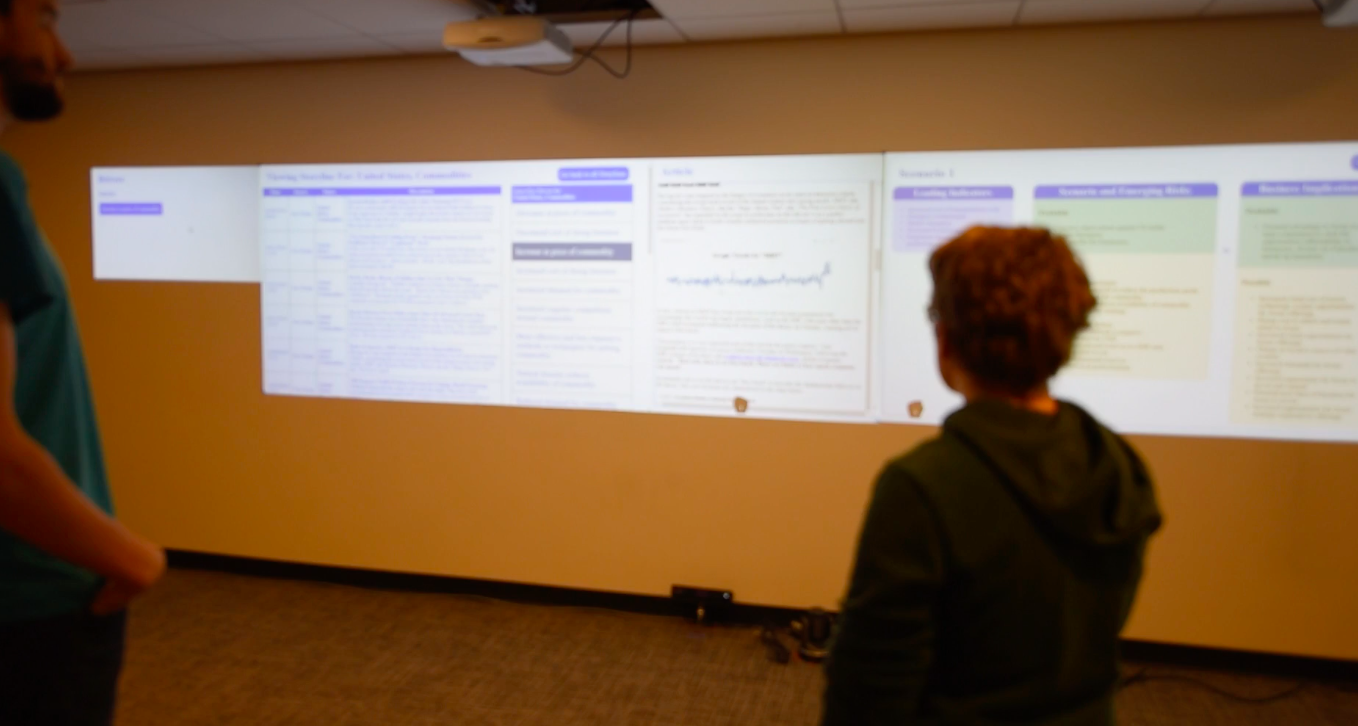
\includegraphics[width=\linewidth]{chapters/02_technology/figures/env_wall.png}
    \end{subfigure}
    \begin{subfigure}[b]{.48\linewidth}
        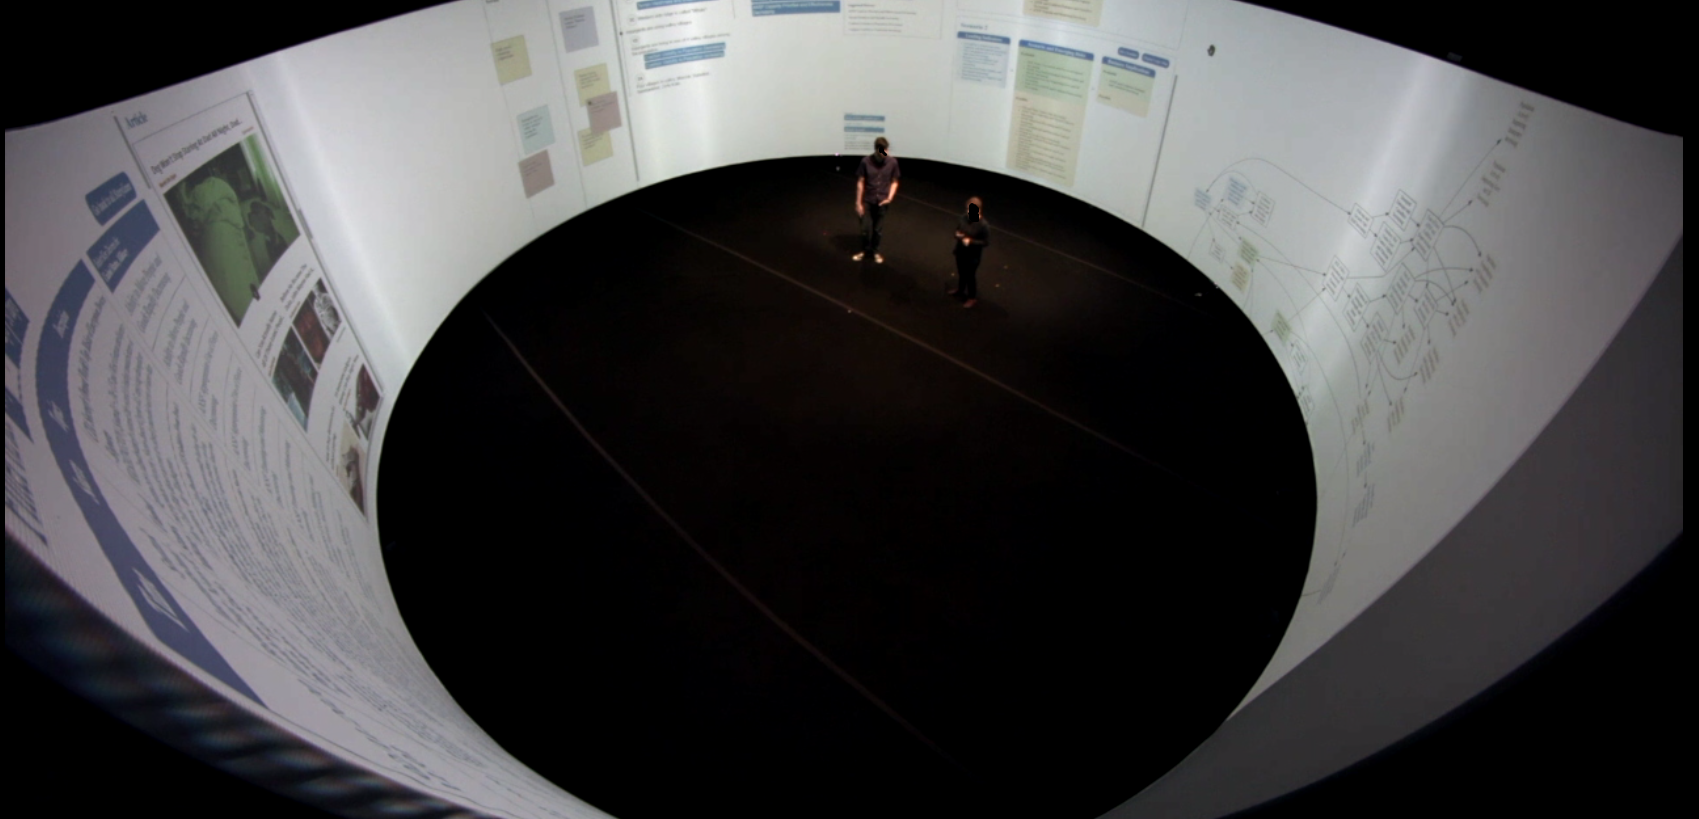
\includegraphics[width=\linewidth]{chapters/02_technology/figures/env_360.png}
    \end{subfigure}
    \caption{Two environments in which we deploy the CAIS, one a long flat wall and the other 360$^{\circ}$ screen.}
    \label{fig:cais_environments}
\end{figure}